\documentclass{kththesis}

\usepackage{blindtext} % This is just to get some nonsense text in this template, can be safely removed
\usepackage{graphicx}
\usepackage{csquotes} % Recommended by biblatex
\usepackage{biblatex}
\usepackage{amsfonts,amssymb,mathrsfs}

\usepackage{float}
\usepackage[colorlinks,
            linkcolor=red,
            anchorcolor=blue,
            citecolor=green
            ]{hyperref}
            
\addbibresource{references.bib} % The file containing our references, in BibTeX format


\title{Adversarial Domain Adaptation for Screening Mammograms}
\alttitle{Detta är den svenska översättningen av titeln}
\author{Tao Wang}
\email{t@kth.se}
\supervisor{Hossein Azizpour}
\examiner{Mårten Björkman}
\programme{Master in Computer Science}
\school{School of Computer Science and Communication}
\date{\today}


\begin{document}


\frontmatter

\titlepage

\begin{abstract}
  English abstract goes here.

%   \blindtext
\end{abstract}


\begin{otherlanguage}{swedish}
  \begin{abstract}
    Swedish abstract goes here.
  \end{abstract}
\end{otherlanguage}


\tableofcontents


% Mainmatter is where the actual contents of the thesis goes
\mainmatter


\chapter{Introduction}


% \Blindtext
% \section{Background}

% \section{Research Question}
% \blindtext
\chapter{Background}
\section{Transfer Learning}
Machine learning has been quite successful in recent years. However, many machine learning methods are based on a common assumption: the training data and the testing data are sampled from a same distribution. When they come from a different distribution, or the distribution changed, the trained model's performance will dramatically decrease. Transfer learning aims to solve this problem, which will transfer the knowledge learned from the original distribution to the new one. Here is how we define the transfer learning in a notation form\cite{pan2010survey}:

\noindent Firstly, let's define \emph{domain}, a \emph{domain} D contains two parts: a feature space  $\mathcal{X}$, a marginal probability distribution $P(X)$. And $X = \{x_1,x_2,x_3,...,x_n\}$, where $x_i \in \mathcal{X}$. 

\noindent Then, when given a domain $D = \{\mathcal{X}, P(X)\}$, a \emph{task} $\mathcal{T}$ is defined as $\mathcal{T} = \{\mathcal{Y},P(Y|X)\}$, where $\mathcal{Y}$ is the label space, and $Y = \{y_1,y_2,y_3,...,y_n\}$, where $y_i \in \mathcal{Y}$. And $P(Y|X)$ means the conditional probability, actually it is an objective predictive function. When given features $X$, our aim is to find the most possible labels $Y$. In the actually work, we need to find an approximate representation of $P(Y|X)$, which is also the goal of machine learning.

\noindent Finally, we can define the transfer learning: given source and target domains $D_S$ and $D_T$, then source and target tasks $\mathcal{T}_S$ and $\mathcal{T}_T$. Transfer learning aims to help improve the performance of $P_T(Y|X)$ in $\mathcal{T}_T$ by using the knowledge learned from $D_S$ and $\mathcal{T}_S$, where $D_S \neq D_T$ or $\mathcal{T}_S \neq \mathcal{T}_T$.

\noindent As we have mentioned that in transfer learning, $D_S \neq D_T$ or $\mathcal{T}_S \neq \mathcal{T}_T$, so the source and target conditions can vary in the following four ways:
\begin{itemize}
    \item $\mathcal{X}_S \neq \mathcal{X}_T$. The target and source domain has different feature space, for example, two documents are written in different language, which will bring different feature space. 
    \item $P_T(X) \neq P_S(X)$. The marginal probability distributions of source and target domain are different. The source and target features are sampled from different distribution. This scenario is called domain adaptation, which is the main focus in our paper. 
    \item $\mathcal{Y}_T \neq \mathcal{Y}_S$. The label space are different. In the actually application of transfer learning, this scenario is rare. 
    \item $P_T(Y|X) \neq P_S(Y|X)$. The conditional probability distributions of source and target are different. This scenario is also very common. But we do not focus on this problem in our project.
\end{itemize}

\section{Domain Adaptation}
\subsection{Definition}
Domain adaptation is one of the sub questions of transfer learning. Domain adaptation tried to build a model which is suitable on both source and target domain. The notation definition is:  given source and target domains $D_S$ and $D_T$, then source and target tasks $\mathcal{T}_S$ and $\mathcal{T}_T$. Domain adaptation aims to help improve the performance of $P_T(Y|X)$ in $\mathcal{T}_T$ by using the knowledge learned from $D_S$ and $\mathcal{T}_S$, where $P_S(X) \neq P_T(X)$ and $P_S(Y|X) \approx P_T(Y|X)$.

\paragraph{Covariate shift}~{}\\
Shimodaira et al.\cite{shimodaira2000improving} first proposed the concept of covariate shift, which is an important concept in domain adaptation. As we have already know that the source and target task's conditional probability distribution are same, then the difference between these two domains is called covariate shift. Shimodaira et al.\cite{shimodaira2000improving} defined \emph{misspecified} models to indicate the influence of covariate shift in model training. Although $P_S(Y|X) \approx P_T(Y|X)$ appears sweet, in the real world application, what we usually find is $P(Y|X,\theta)$. We optimize the parameter $\theta$ to minimize the expected classification error. But it is hard to find a parameter $\theta^*$ which could fit $P(Y|X,\theta^*) = P(Y|X)$ for all $x \in \mathcal{X}$. So the model $P(Y|X,\theta^*)$ we find is called a \emph{misspecified} model. The model's parameter $\theta^*$ is depend on $P(X)$. The difference between $P_S(X)$ and $P_T(X)$ will bring the difference between the model trained from source domain and the one from the target domain. 

\paragraph{Single Good Hypothesis}~{}\\
We usually believe that there exists a model or hypothesis $H^*$, making the error on source domain $E_S(H^*)$ and the error on target domain $E_T(H^*)$ are both small. 

\paragraph{Domain discrepancy and Error}~{}\\
Domain discrepancy is used to describe the difference between the source and target domain. Usually the smaller domain discrepancy is, the better performance we will get in the final model. 

% \subsection{More...}

\section{Generative Model}
The goal of generative model is finding a function used to approximate fit the distribution of the original data. If we use $f(X;\Theta)$ represents such a function, so finding the parameter $P(\Theta)$ is a process of maximum likelihood estimation. The question is when the data distribution is complex, our $f$ will also be complex. And deep neural network could be used to represent such a complex function. There are two successful frameworks used to build a generative model: variational auto-encoder(VAE) and Generative Adversarial Network(GAN). In this project we mainly focus on the GAN. 

\subsection{Variational Autoencoders}
Variational Autoencoders\cite{kingma2013auto,doersch2016tutorial}(VAE) is designed based on encoder-decoder structure. Usually we will have a observed data x, for example an image and this observed data is generated by a latent code z. So training a encoder is trying to find a $q_{\phi}(z|x)$ and training a decoder is trying to find a $p_{\theta}(x|z)$. The training goal of the VAE is to maximize the following likelihood function:
\begin{equation}
    \log_{\theta}(x^{(1)},x^{(2)},...,x^{(N)}) = \sum_{i=1}^{N}\log p_\theta(x^{(i)})
\end{equation}

Now we can use the $q_{\phi}(z|x^{(i)})$ to approach the posterior of $p_{\theta}(z|x^{(i)})$. To estimate the similarity between these two distribution, we use Kullback-Leibler divergence to describe it.

\begin{eqnarray}
KL(q_{\phi}(z|x^{(i)})||p_{\theta}(z|x^{(i)})) &=& \mathbb{E}_{q_{\phi}(z|x^{(i)})} \log \frac{q_{\phi}(z|x^{(i)})}{p_{\theta}(z|x^{(i)})} \nonumber \\
&=& \mathbb{E}_{q_{\phi}(z|x^{(i)})} \log \frac{q_{\phi}(z|x^{(i)})p_{\theta}(x^{(i)})}{p_{\theta}(z|x^{(i)})p_{\theta}(x^{(i)})} \nonumber \\
&=& \mathbb{E}_{q_{\phi}(z|x^{(i)})} \log \frac{q_{\phi}(z|x^{(i)})}{p_{\theta}(z,x^{(i)})}+\mathbb{E}_{q_{\phi}(z|x^{(i)})} \log p_{\theta}(x^{(i)}) \nonumber \\
&=& \mathbb{E}_{q_{\phi}(z|x^{(i)})} \log \frac{q_{\phi}(z|x^{(i)})}{p_{\theta}(z,x^{(i)})}+ \log p_{\theta}(x^{(i)}) \nonumber \\
&=& \mathbb{E}_{q_{\phi}(z|x^{(i)})} \log \frac{q_{\phi}(z|x^{(i)})}{p_{\theta}(z)} -\mathbb{E}_{q_{\phi}(z|x^{(i)})} \log(p_{\theta}(x^{(i)}|z)) + \log p_{\theta}(x^{(i)}) \nonumber \\
&=& KL(q_{\phi}(z|x^{(i)})||p_{\theta}(z)) -\mathbb{E}_{q_{\phi}(z|x^{(i)})} \log(p_{\theta}(x^{(i)}|z)) + \log p_{\theta}(x^{(i)}) \nonumber
\end{eqnarray}

So 
\begin{equation}
    \log p_{\theta}(x^{(i)}) = \mathbb{E}_{q_{\phi}(z|x^{(i)})} \log(p_{\theta}(x^{(i)}|z))+ KL(q_{\phi}(z|x^{(i)})||p_{\theta}(z|x^{(i)})) - KL(q_{\phi}(z|x^{(i)})||p_{\theta}(z))
\end{equation}

This is a basic equation of VAE. And $KL(q_{\phi}(z|x^{(i)})||p_{\theta}(z|x^{(i)}))$ is non-negative. If $q_{\phi}(z|x^{(i)})$ and $p_{\theta}(z|x^{(i)})$ are totally equal, this term will be zero. So we could turn to optimize the
\begin{equation}
     \sum_{i=1}^N\mathbb{E}_{q_{\phi}(z|x^{(i)})} \log(p_{\theta}(x^{(i)}|z)) - KL(q_{\phi}(z|x^{(i)})||p_{\theta}(z))
\end{equation}
instead of $\sum_{i=1}^N p_\theta(x^{(i)})$.

The first term could be optimized by stochastic gradient descent and using minibatch training samples. This term could be viewed as reconstruction error by using L2 loss. And the second term similarly, $p(z)$ could be viewed as a normal distribution $N(0,1)$, and the encoder $q_{\phi}(z|x)$'s output is the mean and the variance of the normal distribution want to approximate. The training process could also be done by backpropagate algorithm. 

Variational Autoencoders is quite efficient in generating samples, while VAE usually tend to result in blurry images\cite{doersch2016tutorial} because of the pixel-wise reconstruction losses.
\subsection{Generative Adversarial Network}
Generative Adversarial Network(GAN) was proposed by Ian Goodfellow\cite{goodfellow2014generative} inspired from two-player game. The role of this two player in GAN is generative model and discriminative model. Following graph shows the structure of GAN.

\begin{figure}[H]
    \centering
    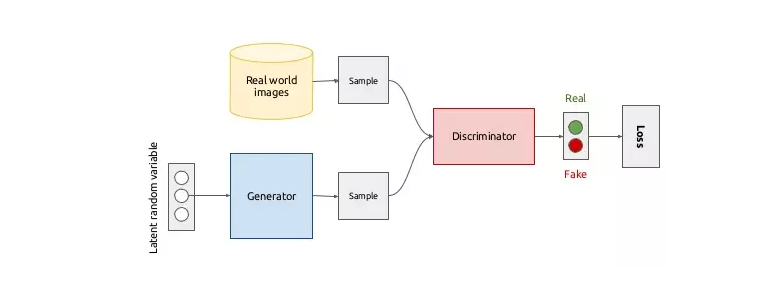
\includegraphics[scale = 0.6]{GAN.png}
    \caption{GAN's structure used in computer vision}
\end{figure}

\noindent Generative model is used to simulate the real world data's distribution, and the discriminative model is a binary classifier, used to classify the fake and the real data. A generator receive a random noise and generate a fake picture, and a discriminator tries to judge whether this picture is fake or not. The goal of the generator is to confuse the discriminator, while the discriminator aims to resist this confusion. Here is the representation of this minmax game:
\begin{equation}
    \min \limits_G \max \limits_D V(D,G) = E_{x\sim P_{data}}[log(D(x)] +  E_{z\sim P_{z}}log(1-D(G(z)) 
\end{equation}

\noindent In this function, $P_{data}$ is the real data's distribution, and the $P_{z}$ is the fake distribution simulated by generator. $z$ is the input noise. And usually the training method for GAN is mini-batch gradient descent. So the loss function for each m size batch on discriminator D and generator G is:
\begin{equation}
    L_D = \frac{1}{m}\sum_{i=1}^m[-log(D(x^{(i)}) -  log[1-(D(G(z^{(i)}))] 
\end{equation}
\begin{equation}
     L_G = \frac{1}{m}\sum_{i=1}^m log[1-(D(G(z^{(i)}))]
\end{equation}

But the GAN method still faces some practical problem: 
\begin{itemize}
    \item Non-convergence. GAN has a good performance on the Nash equilibrium problem, while the gradient descent method only guarantee the Nash equilibrium on a convex problem. When both of the players is represented by neural network, the perfect equilibrium is hard to achieve, making the network continually update themselves, which brings the non-convergence problem.
    \item Collapse problem\cite{salimans2016improved}. The GAN is a minmax game, so there does not exist a strict loss function. So it is hard to distinguish whether the generator get improved or not. Sometimes the generator will always generate the same point, making the training could not continue, then we call the GAN meets collapse problem. 
    
\end{itemize}

\section{Semantic Segmentation}
Semantic segmentation is understanding an image at pixel level, for example we want to assign each pixel in the image an object class. For example, in the following picture
\begin{figure}[H]
    \centering
    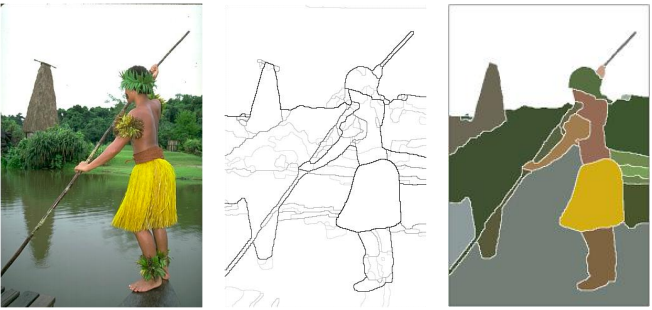
\includegraphics[scale = 0.4]{sem_seg.png}
    \caption{An example of semantic segmentation}
\end{figure}

\noindent Apart from recognizing the man and the background, we also have to delineate the boundaries of each object. Therefore, unlike classification, we need dense pixel-wise predictions from our models.

\chapter{Related work}


% There are mainly two directions in deep domain adaptation:
% One direction is to minimize the difference between the source and target domain. And the other direction is to use adversarial loss to modify the discriminative representation space. 
\section{Adversarial Domain Adaptation}

The proposed of GAN\cite{goodfellow2014generative} has provided domain adaptation a new direction, adversarial domain adaptation. Actually, Hu et al.'s \cite{hu2017unifying} work indicated that GAN is a special case of adversarial domain adaptation with a degenerated source domain. In the following part, we will show some recent study of adversarial domain adaptation.

\subsection{Feature-Level Adaptation}

\paragraph{DANN}~{}\\


\noindent At 2015, \cite{ganin2015unsupervised,ganin2016domain} proposed a model in feature-leveled domain adaptation by using the adversarial method \cite{goodfellow2014generative}: Domain-adversarial Neural Network (DANN), which could be viewed as the birth of adversarial domain adaptation. This model contains three parts: a feature extractor used to extract the feature from the input images, a label classifier used to predict the class label and a domain classifier used to classify the domain label. On one hand, the loss from the domain classifier needs to be minimized in order to correctly distinguish the source and target domain. On the other hand, to find the domain invariant feature, the loss function of the domain classifier needs to be maximized. By formulating such a min-max game, DANN find a common feature space between the source and target. 

\noindent Then, there appear some variants based on DANN. \cite{tzeng2015simultaneous} considered the similarity between the classes, and proposed the soft label loss. \cite{tzeng2017adversarial} used untied weight mapping in feature extractor and reduce the difficult in optimization. 

\paragraph{DSN}~{}\\

\noindent Finding a mapping function or a function or a domain invariant representation, which in principle, is a good idea. \cite{bousmalis2016domain} thinks that these methods will be affected by the different distribution in low level. So Domain Separation Network(DSN) was proposed. DSN not only extract the domain invariant feature but also extract the identity feature of the source and target domain, which could be viewed as the low level features. And from the authors point of view, the invariant feature subspace show be orthogonal with the identity subspace. Also this paper adopted MMD\cite{gretton2012kernel} method and gradient reversal layer\cite{ganin2015unsupervised,ganin2016domain} to train the invariant feature extractor. 

\noindent However, all these approaches is based on feature level and started with a feature extractor layer, which does not enforce any semantic consistency\cite{hoffman2017cycada}. 

\subsection{Pixel-Level Adaptation}

Pixel-Level domain adaptation is usually combined with image generation or style transfer. The task of pixel-level adaptation is not only focus on a correct classification but also on generating a picture with a clear semantic meaning. Also, There are several works about the pixel-level adaptation based on GAN in recent years. 

\paragraph{PixelDT}~{}\\

\noindent Yoo\cite{yoo2016pixel} studied the domain transfer problem. They tried to achieve a domain transfer of clothes on semantic level. They build a three levels network. The first level is called convert, which is build by an encoder and a decoder. Encoder firstly extract the low-level semantic information of a source picture, and the decoder decode this information into another picture. Actually, the encoder is a convolutional neural network, and we will use the second and third level network to train the decoder. The second level is a real/fake discriminator and the third level is a domain discriminator. The decoder tried to confuse the real/fake discriminator, making the decoder result look natural and it tried to confuse the domain discriminator, making the decoder result come from the target domain. 

\paragraph{PixelDA}~{}\\


\noindent Bousmalis et al.\cite{bousmalis2016unsupervised} did a study about the domain adaptation on the pixel-level. They got inspiration from the style transfer \cite{gatys2016image,johnson2016perceptual} using GAN. Except from using domain loss and task loss like some feature-level domain adaptation\cite{ganin2015unsupervised,ganin2016domain,tzeng2017adversarial}, they also proposed a content-similarity loss on the pixel-level. Different from the style transfer, this model PixelDA aims to learn the style of the whole source domain. By learning the style of the source on pixel-level, the model could decouple from the task-specific architecture and has a higher training stability. 

\paragraph{CoGAN}~{}\\

\noindent Coupled Generative Adversarial Networks\cite{liu2016coupled} was used to learn the joint distribution of multi-domain images. The method of CoGAN is simple, by training two GANs at the same time, and there are some layers shared between these GANs. In the generator, the first several layers shared the weight, and in the discriminator the last several layers shared the weight. From this paper's view, we could extract the invariant features, for example the object contour, and by the first several layers and in these private layers, we could get some detail information, such as texture. So the final loss function is the combine of these identical GAN's loss function, and the training method is as same as the DCGAN's \cite{radford2015unsupervised} training method. 

\paragraph{pix2pix}~{}\\

\noindent Isola et al.\cite{isola2016image} studied the image-translation problem, they build a image-to-image translation fromework(pix2pix) based on conditional adversarial networks\cite{mirza2014conditional}. They add a L1 term into loss function, making the generator's task is not only fooling the discriminator but also being near the ground truth output in an L1 sense. The authors thinks comparing with L2 term, L1 could encourage less blurring. Also different from the traditional encoder-decoder structure, the structure is based on U-net\cite{ronneberger2015u}, which is an skip encoder-decoder with skip connections between mirrored layers in the encoder and decoder stacks. While in discriminator, we need to concern about both high and low level correctness. So the author proposed a PatchGAN method, by splitting the image into several N$\times$N patches.The final discriminator result is the average of these patches results. 

\paragraph{CycleGAN}~{}\\

\noindent No matter how impressive the pix2pix structure's result is, this framework is based on cGAN, which means the input images are paired. Zhu et al.\cite{zhu2017unpaired} used cycle-consistent adversarial network(CycleGAN) to finish an unpaired-image translation on pixel-level. When doing adversarial domain adaptation, usually we can not find the low level corresponding relationship. While CycleGAN adopts another generator, which tried to convert the generated picture into the source picture and add such cycle consistent loss into the loss function. Similarly, DiscoGAN\cite{kim2017learning}, DualGAN\cite{yi2017dualgan} were based on the same method. The only difference is DualGan change traditional GAN into Wasserstein GAN\cite{arjovsky2017wasserstein} to improve the stability and DiscoGAN chosse L2 for cycle consistency, while DualGan and CycleGAN choose L1 for cycle consistency. 

\paragraph{UNIT}~{}\\

\noindent Liu et al.\cite{liu2017unsupervised} combine the VAE\cite{kingma2013auto,rezende2014stochastic}, coGAN and CycleGAN together and get a network called Unsupervised Image-to-Image Translation Networks(UNIT). Such framework also based on a shared latent space assumption. So UNIT firstly use a VAE to map the images from different source into a same latent space. KL divergence terms is used to penalize deviation of the distribution of the latent code from the prior distribution. Then, similar with what we did in coGAN, for each domain, we used a partly weight shared generator and a totally identical discriminator. To make the generator learn the domain specific feature, we use a cycle-consistent loss function, by comparing the generated pictures and the original pictures. So the final method is using VAE get the latent code and using coGAN to re-generate the pictures from the latent code. We can just simply change the generate and discriminator to achieve a domain transfer. The similar structure and method are also used in XGAN.\cite{royer2017xgan}

\paragraph{CyCADA}~{}\\

\noindent Hoffman et al. \cite{hoffman2017cycada} make a improvement named cycle-consistent adversarial domain adaptation(CyCADA) based on \cite{zhu2017unpaired}. They proposed that there are three kind of loss during domain adaptation: pixel loss, feature loss, semantic loss. Also they also adopted cycle consistent like\cite{zhu2017unpaired} to learn an invertible mapping function. Different from the style-transfer\cite{gatys2016image,johnson2016perceptual}, they defined a semantic loss instead of content loss. Content loss is calculated from pixel to pixel, while semantic loss in this paper is represented by the sum of the classification loss on both fake picture and the inverted picture. And the author insist that these two representation are analogous. 

\paragraph{StarGAN}~{}\\

\noindent While their is still a big problem in CycleGAN and its variants: CycleGAN is only suitable for the two domain problem, when we are facing multi-domains question, we need to build a model for each two domain. Choi et al.\cite{choi2017stargan} seems find an approach to solve the multi-domain problem: StarGAN. The method behind StarGAN is simple, instead of finding a mapping function between each two domains, StarGAN tried to find a mapping function between each domain and a common domain. Also they use mask vector to build a uniform domain label space. To stabilize the training process and generate higher quality images, the authors chose Wasserstein GAN\cite{arjovsky2017wasserstein} instead of GAN. 

\paragraph{DTN}~{}\\

\noindent Domain Transfer Network\cite{taigman2016unsupervised} is another important work in adversarial domain adaptation. The authors think that when GAN reaches a balance, the generator gets knowledge from the source domain, and its generated result is indistinguishable for any discriminator, which means the GAN has learned a invariant representation of the source domain. The author creatively add a new loss called identity loss. When we input the generated image into the generator, identity loss will estimate the similarity between such fake input and its output, to guarantee that for a fake input, the output tend to be this original fake input. The generator's structure is similar with Yoo's\cite{yoo2016pixel} method, by encoding the picture into a low level information and then decode it into another picture. 


\paragraph{DRCN}~{}\\

\noindent Deep Reconstruction-Classification Networks\cite{ghifary2016deep}(DRCN) is another network structure used in domain adaptation. DRCN is made by one traditional classification pipeline(an feature extractor and a feature classifier) and another reconstruction pipeline(from extracted feature back to image). DRCN is trained by minimizing the reconstruction error and the classification error on source domain. The author thinks that once we minimize these two errors, the extracted feature would find a domain adaptive representation for both source and target domain. Also to improve the performance of DRCN, the author adopted data augmentation and denoising autoencoders to improve the generalization ability.

\paragraph{FADA}~{}\\

\noindent In supervised domain adaptation, usually we will face a problem that there are only few labelled target example, Few-Shot Adversarial Domain Adaptation(FADA)\cite{motiian2017few} provides us a solution. The main method of this paper is to learn an embedded subspace which maximizes the confusion between source and target domains while semantically aligning their embedding. The author thinks that in unsupervised domain adaptation, especially the domain adaptation using adversarial method, we need to align the distributions, but the distributions alignment can not always guarantee to achieve a semantic alignment, which the author thinks is a major source of performance reduction. So the main innovation of this paper is introducing a domain-class discriminator(DCD), which is a two fully connected layer with a softmax activation in the last layer, used to align the semantic level meanings in source and target domain.

\section{Deep Semantic Segmentation}
Semantic Segmentation is a classical computer vision problem. With the development of deep learning technology, semantic segmentation could achieve a more accurate result. In the following part, we will show some recent study of semantic segmentation.

\paragraph{FCN}~{}\\
\noindent Fully connected network(FCN) was proposed by Long et al.\cite{long2015fully}. The structure of FCN is based on traditional CNN. By using FCN we could classify each pixel's class. Usually a CNN will add several fully connected layers after the convolution layers. While in FCN, we will use the convolution layers to instead these fully connected layers. And FCN will use the upsampling method to upsample these convolution layers back to the original size. And also skip architecture is used in FCN to optimize the result.

\paragraph{SegNet}~{}\\
\noindent SegNet\cite{badrinarayanan2017segnet} is another network based on FCN, which is used for autopilot. The structure of SegNet is also encoder-decoder structure, the encoder part is a pre-trained VGG-16\cite{simonyan2014very} network. The difference with FCN is the way how the SegNet do the up-sampling process. In SegNet, when doing the pooling process, the network will store the pooling indices and in decoder the up-sampled is based on these pooling indices. While in FCN, the up-sampling method is tried to find a deconvolution function and sum the up-sampling result with the encoded feature map. 

\paragraph{U-Net}~{}\\
\noindent However, the FCN is based on millions of training images, which is hard to achieve in a biomedical task. So here comes U-net\cite{ronneberger2015u}. The structure of U-net is similar with FCN, but different from FCN, U-Net does not use pre-trained CNN model\cite{simonyan2014very}, because U-net is usually used in binary classification. And in lower level feature fusion part, U-net concat the original feature with the up-sampled feature. Also the author mentioned that they also use data augmentation to solve the limited training data problem.  

\paragraph{DeepLab}~{}\\
DeepLab\cite{chen2016deeplab} is a popular semantic segmentation framework, which made some improvements based on FCN. First of all, while doing up-sampling in FCN, the existence of stride will bring the decrease of the resolution in the result. So in deeplab framework, we will set stride to one and also adopted dilated convolutions\cite{yu2015multi} strategy, to avoid the shrink of the result size. Secondly, the FCN is basically a encode-decode process, which will absolutely bring the loss of the information. So deeplab used a fully connected conditional random field\cite{krahenbuhl2011efficient} together with a bilinear interpolation to refine the segmentation result. 


\chapter{Methods}

% \blindtext

\printbibliography[heading=bibintoc] % Print the bibliography (and make it appear in the table of contents)

\appendix

\chapter{Unnecessary Appended Material}

\end{document}
